\chapter{Packrat Proxies}
\label{sec:packrat}

This chapter describes and evaluates new techniques for
network-originated retransmissions for end-to-end transport
connections, yielding performance benefits for encrypted transport
protocols in lossy settings.  We use the IBLT quACK from \Cref{sec:quack}
to let the receiver efficiently acknowledge
encrypted packets to a network function, without modifying the sender
or the underlying wire format. With these tools, endpoints can receive
network-originated retransmissions appropriate for them, without an
additional layer of encapsulation, tunnel, or link-layer
retransmissions.

\section{Introduction}
\label{sec:packrat:intro}

The relationship between Internet transport protocols and lossy
wireless networks has long been fraught. Three decades ago, the
seminal Snoop work~\cite{balakrishnan1995snoop} addressed an issue
that emerged with the rise of wireless Ethernet (Wi-Fi): TCP's
end-to-end reliability works poorly over network segments that
regularly experience non-congestive packet loss. This is for two big
reasons: it's wasteful to require frequent end-to-end retransmissions
over a whole network path to address packet loss on one wireless link,
and because most congestion-control schemes interpret packet loss as a
sign of congestion and will slow down in response---a mistake when the
loss wasn't caused by congestion. From its point of view in 1995, the
Snoop paper outlined three plausible solutions:

\begin{itemize}[noitemsep]
\item \textbf{Splitting TCP connections}~\cite{bakreitcp1994, bb95}. A
  proxy at the wireless base station transparently interposes on TCP
  connections that cross it, creating two concatenated connections:
  one from ``fixed host'' to proxy, and from proxy to the ``mobile
  host.'' This lets retransmission occur over the lossy segment only,
  and prevents the fixed host's congestion control from seeing
  non-congestive wireless losses.

\item \textbf{Link-level acknowledgment and
  retransmission}~\cite{palplus}. Wireless NICs add their own
  encapsulation (with their own sequence numbers or packet
  identifiers) to each packet, reply to incoming packets with
  link-layer acknowledgments, detect apparent losses from the absence
  of an ACK, and retransmit lost packets before the end-to-end
  transport protocol concludes they were lost.

\item \textbf{The Snoop approach}, where an on-path network function
  transparently interprets TCP acknowledgments in-flight, detects
  losses, retransmits packets over the lossy link only, and
  temporarily hides loss from the other host to avoid a duplicate
  retransmission.
\end{itemize}

In the intervening years, the first two approaches were widely
deployed. At the boundary between the wired Internet and a lossy
wide-area subpath (e.g.~a satellite or cellular network), network
operators used connection-splitting performance-enhancing proxies
(PEPs) to accelerate TCP connections crossing their networks. For
lossy \emph{local}-area subpaths, Wi-Fi and cellular networks use
link-layer sequence numbers, selective ``block'' acknowledgments,
link-layer retransmissions, and receiving NICs that sometimes hold
back received packets to wait for retransmissions of earlier packets
so that hosts receive packets in the original order to avoid
triggering a transport-layer end-to-end retransmission~\cite{rfc3366,
  rfc8985, ieee802.1ac, 5Greorder}. Because of the practical success of
the first two approaches, Snoop's ``network-originated
retransmissions'' didn't seem to be needed in practice.

Until, we propose, maybe now. Post-TCP transport protocols,
especially QUIC~\cite{rfc9000}, encrypt and authenticate their
packets. This puts some operators in a bind, because they can no longer
``split'' these connections.
But what about link-layer ACKs and retransmissions?
This is a usable strategy on low-latency wireless links when one party
(or standards body) controls both sides, and losses can be patched
before the end-to-end protocol detects them. But when the lossy
subpath has higher latency (as for some satellite or experimental
networks), losses can't be patched before the transport protocol
detects them, and the head-of-line blocking necessary to put
packets back in order at the receiver can be ruinous to real-time
applications. In any event, such techniques can't be deployed
unilaterally by a network operator who doesn't control the receiver or
the encapsulation format.

What else could address this? Traffic sources could deploy
congestion-control and loss-detection schemes that are less sensitive
to loss and reordering~\cite{rfc8985}, but this is also out of a
network operator's control. Yet another approach could involve
Sidekick proxies (\Cref{sec:sidekick})---but these provide
in-network \emph{acknowledgments} of encrypted transport protocols
(for hosts to interpret and perhaps trigger retransmission), not
in-network \emph{retransmissions} based on the encrypted traffic of
hosts.

Given all this, what really happens today, at least some
of the time, is that satellite and other nontraditional network
operators block QUIC traffic, forcing hosts to fall back to TCP that
can be split as before. We think it may be possible to do better by drawing on ``Snoop-style''
ideas. In this chapter, we describe and evaluate Packrat\footnote{For
``packet rateless retransmission''---and because the Packrat proxy keeps
a small cache of recent packets-in-flight for possible retransmission.}
protocols: a technique for network-originated retransmissions for encrypted
end-to-end transport connections, yielding performance benefits in lossy
settings. We adapt the set reconciliation techniques from \Cref{sec:quack} to
let the receiver efficiently acknowledge encrypted packets (in a ``quACK'') to
a network function, without modifying the sender or the underlying wire format.
Compared to the power sum quACKs used by Sidekick protocols
in \Cref{sec:sidekick}, IBLT quACKs are faster to decode. This makes them more
appropriate for a deployment where network functions are the ones interpreting
acknowledgments over encrypted sequence numbers from many connections in
parallel and triggering retransmissions as a result.

We integrate the Packrat proxy with several applications built on encrypted
transport protocols, and show that it can enable a variety of performance
enhancements in settings with a lossy path segment near the data receiver,
compared to end-to-end loss recovery schemes:

\begin{enumerate}[noitemsep]
\item Application 1: Improved throughput for large file downloads using QUIC and HTTP/3.
\item Application 2: Reduced packet tail latency of a low-latency media stream using a simple repetition code.
\item Application 3: Reduced end-to-end retransmissions at the server of a reliable multicast RTP stream.
\end{enumerate}

\begin{figure}[t]
    \centering
    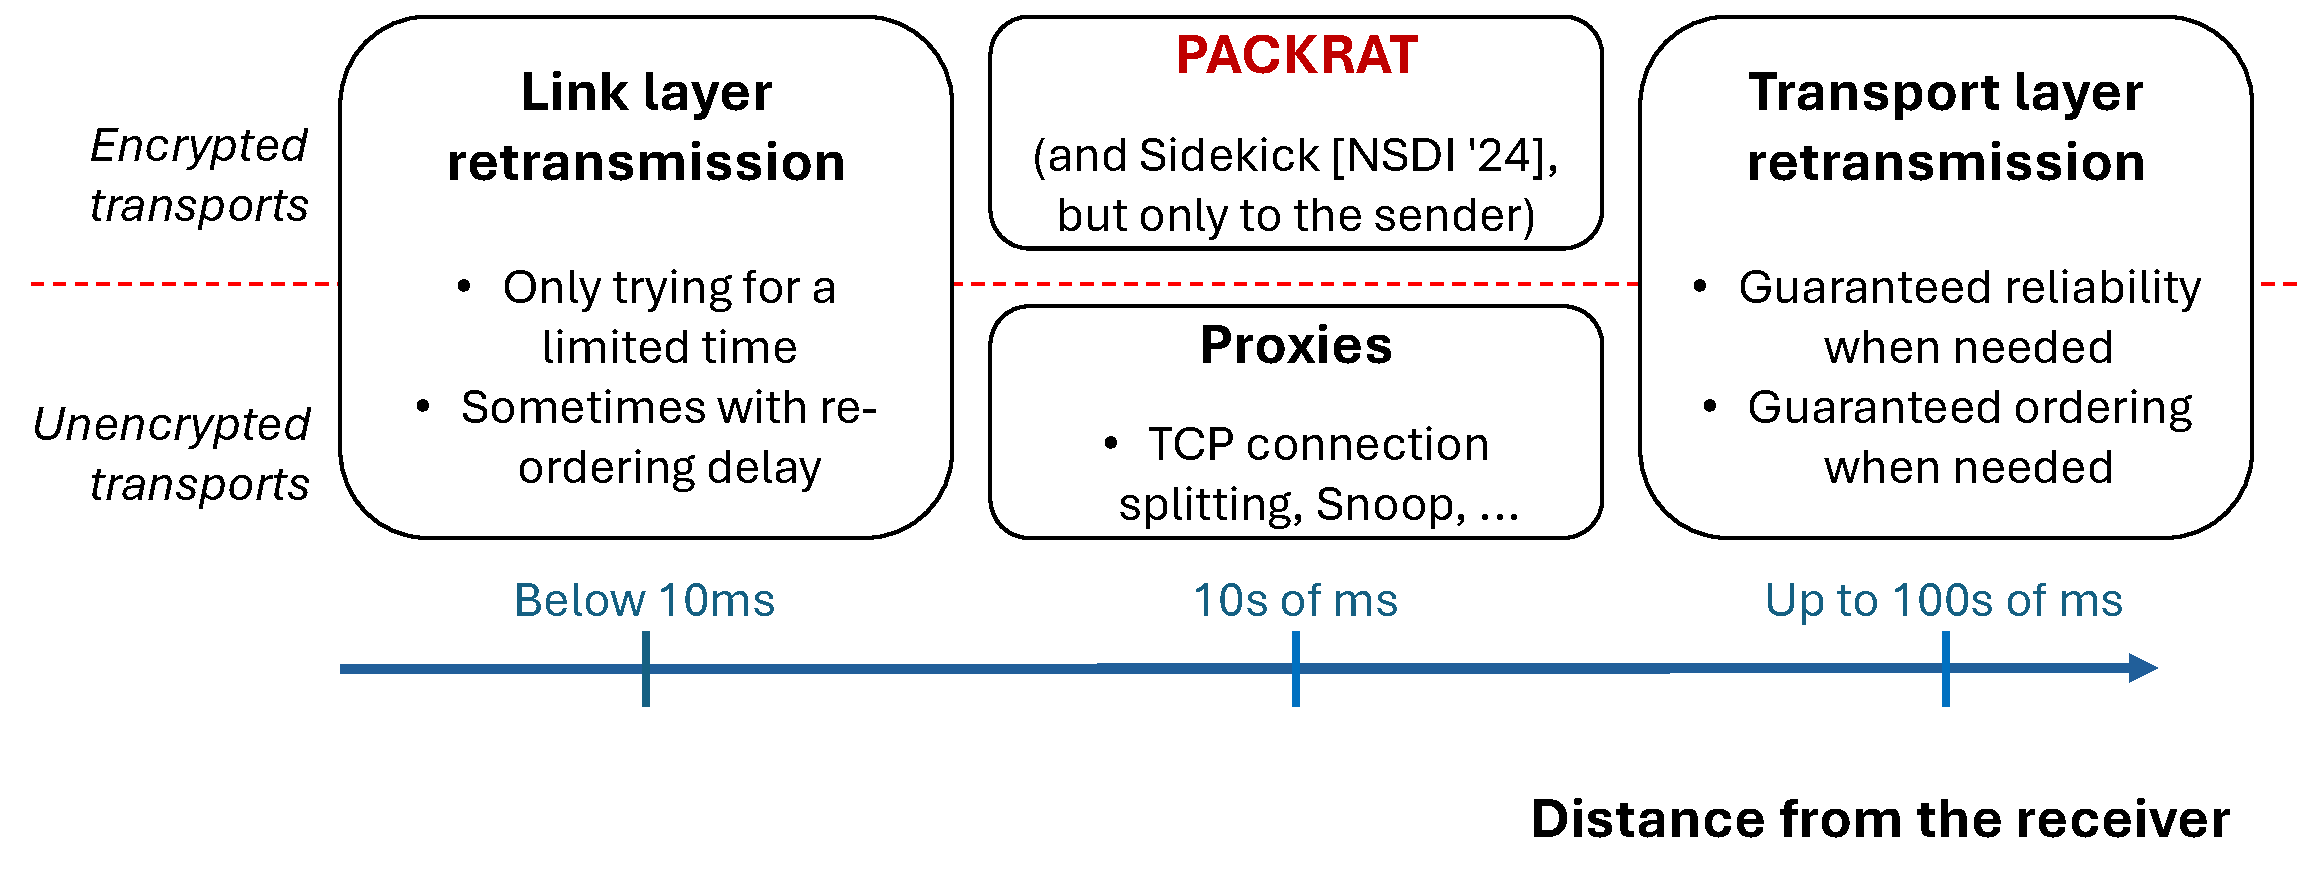
\includegraphics[width=0.9\linewidth]{packrat/figures/packrat-scope.pdf}
    \caption{The scope of Packrat compared to other methods for in-network retransmissions.}
    \label{fig:packrat:packrat-scope}
\end{figure}

\noindent \Cref{fig:packrat:packrat-scope} shows the scope of Packrat compared
to other methods of in-network retransmissions over lossy path segments.
Unlike link-layer retransmissions, the assistance from a Packrat can be
deployed anywhere along the network path and tailored to the performance
demands of each base connection. Compared to existing transport-layer
solutions, Packrat can be applied to arbitrary transport protocols without
ossification.

\subsubsection{Summary of results.}
To summarize, we show that it is possible to provide per-connection in-network
retransmissions to secure transport protocols along an adjacent connection
using Packrat proxies, without involving the data sender nor modifying the
wire format of the underlying connection. We start with a brief history of loss
recovery in the network (\Cref{sec:packrat:background}), then describe our
contributions:

\begin{itemize}[noitemsep]
    \item A mechanism at the \textit{endpoint} to correct
     end-to-end reordering signals when there are in-network retransmissions
     (\Cref{sec:packrat:problem}).
    \item The use of Packrat proxies with an adjacent Sidekick connection, and
     optimizations to improve compute scalability based on the co-location of
     the endpoint and quACK sender(\Cref{sec:packrat:design}).
    \item An implementation of the Packrat proxy and integrations with three
     applications that use encrypted transport (\Cref{sec:packrat:implementation}).
    \item An emulation study of the performance enhancements, as well as the CPU,
     memory, and link overheads of using a Packrat proxy.
     (\Cref{sec:packrat:methodology,sec:packrat:emulation}).
\end{itemize}

\noindent Finally, we conclude (\Cref{sec:packrat:summary}).

\section{Background: In-network retransmissions}
\label{sec:packrat:background}

We provide a brief history of loss recovery mechanisms in the network to
motivate the need for lightweight, non-ossifying, in-network retransmissions
for secure transport protocols.

\subsubsection{End-to-end loss recovery.}

In end-to-end loss recovery,
congestion control algorithms were traditionally designed to treat all loss as an indicator of
congestion~\cite{rfc5681tcp,rfc2001tcp}.

With modern wireless networks and higher bit-error rates, recent developments
such as the BBR congestion control
% (Bottleneck Bandwidth and Round-trip propagation time)
algorithm have de-prioritized packet loss as a congestion
signal~\cite{cardwell2017bbr}. This change enables higher throughput but has
raised concerns regarding TCP fairness~\cite
{ware2019modeling,philip2024prudentia}. In response, the performance of newer
versions of BBR has regressed in lossy environments, suggesting a lasting trend
in the treatment of loss as a congestion signal regardless of its source~\cite
{yuan2025internet}.

\subsubsection{Link-layer loss recovery.}

Loss recovery at the link layer~\cite{3gpp5gstandard,le2022link,ieee80211e} can
mitigate some of the dramatic reactions of CCAs by hiding random loss from
endpoints.
Applications and transport protocols are oblivious to this
functionality, and there is a tradeoff to this reliability~\cite{klingler2018impact,kliazovich2012arqproxy}.
Retransmitting more often increases the chance
of success but increases the time needed, and may also introduce
jitter and reordering~\cite{leung2007overview}.
Low-latency applications may prefer to transmit new data instead, but
retransmitting less often means more loss.
There is no ideal configuration for all connections that share the link.

\subsubsection{Transport-specific mechanisms.}

Some transport-layer proxies split a connection into two or more segments
and optimize the connection for each segment. In addition to
TCP connection splitters~\cite{rfc3135,honda2011still,hayes2019mmwave},
selective forwarding units (SFUs) are
used for media streams where low-latency is critical, so retransmissions occur
closer to the data receiver~\cite{rfc7667,andre2018comparative}.

With Snoop~\cite{balakrishnan1995snoop}, it is clear
that complexities emerge in how the proxy interprets
and modifies plaintext sequence numbers on the wire, which also ossifies TCP.
This chapter aims to explore how such a proxy can send helpful in-network
retransmissions to a variety of encrypted protocols while preserving
end-to-end semantics, without access to such information.

These types of approaches make unwarranted assumptions about
transport headers ossify the protocol~\cite{papastergiou2017deossifying}.
By making reliability guarantees to the endpoint, the connection-splitting
proxies also fate share with the connection.

\subsubsection{Protocol-agnostic transport assistance.}

Forward error correction can be used in lossy environments, but this
introduces significant overheads as entire packet contents (and not just
sequence numbers) must be encoded during transmission~\cite
{rfc9265}. FEC also requires participation from both endpoints.

Mechanisms that encapsulate packets offer potential for reliability without
decrypting packet contents, but their primary focus tends to be security. VPNs
introduce a costly encryption layer. MASQUE tunnels protocols over HTTP/3, and
if used for local retransmissions has the potential for complex nested loss
recovery and congestion control interactions~\cite
{rfc9298,schinazi-masque-proxy-05,kramer2021masquepep}. It is intended to
function per-application, and the best known implementation from Apple
functions like a VPN~\cite{icloud-private-relay}. These proxies may also not be
on-path, which harms performance.

The Sidekick proxy provides protocol-agnostic assistance by sending
``quACKs'' of encrypted packets to an endpoint, but cannot retransmit
packets itself (\Cref{sec:sidekick}). This limits its usefulness
to when the loss is near the data \textit{sender}.
However, client traffic (which is near the lossy last-mile) is typically heavier
in the downlink direction. In this chapter, we similarly leverage set
reconciliation in quACKs for referring to encrypted packets,
but to send network-originated retransmissions.

\section{The reordering problem and spurious retransmissions}
\label{sec:packrat:problem}

\begin{figure}
    \centering
    \begin{subfigure}[b]{0.8\linewidth}
        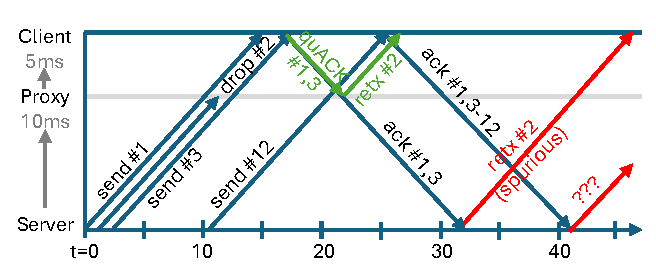
\includegraphics[width=\linewidth, trim=0 10 0 10, clip]{packrat/figures/reordering_unmodified.pdf}
        \caption{Unmodified ACK.}
        \label{fig:packrat:reordering:unmodified}
    \end{subfigure}
    \begin{subfigure}[b]{0.8\linewidth}
        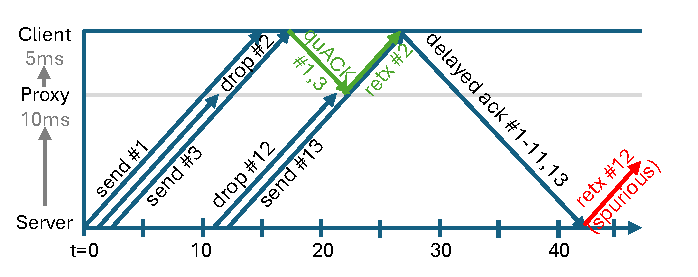
\includegraphics[width=\linewidth, trim=0 9 0 10, clip]{packrat/figures/reordering_delayed_ack.pdf}
        \caption{Na\"ive delayed ACK.}
        \label{fig:packrat:reordering:delayed-ack}
    \end{subfigure}
    \begin{subfigure}[b]{0.8\linewidth}
        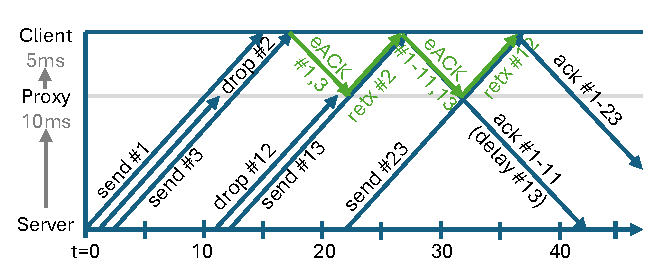
\includegraphics[width=\linewidth, trim=0 9 0 10, clip]{packrat/figures/reordering_with_signal.pdf}
        \caption{ACK with Packrat reorder delay of 10 ms.}
        \label{fig:packrat:reordering:packrat}
    \end{subfigure}
    \caption{The reordering problem where in-network retransmissions with
    millisecond RTTs cause the server to send spurious retransmissions. The
    end-to-end ACKs constructed with a Packrat reorder delay prevent this problem.
    \gina{change eACK to quACK}
    }
    \label{fig:packrat:reordering}
\end{figure}


Most acknowledgment schemes allow for some reordering but not at the level
incurred by in-network retransmissions. For example, TCP fast retransmit requires
three duplicate ACKs~\cite{rfc5681tcp}. The QUIC RFC specifies a threshold of three
out-of-order packets before detecting loss~\cite{rfc9002quic}. The RACK-TLP algorithm
allows for a time-based ``reordering window'', but still penalizes excessive
reordering~\cite{rfc8985}. Compared to, e.g., Wi-Fi retransmits, the
reordering from in-network transmissions is directly related to the RTT to
the proxy on the order of tens of milliseconds.
We call this the \textit{reordering problem}.

Consider an example using selective ACKs, where a gap is considered a missing
packet (\Cref{fig:packrat:reordering:unmodified}): The server sends 1250-byte packets at 10 Mbit/s,
which is 1 packet every ms. The client drops packet \#2 but
receives \#1, \#3, \#4, etc. If the RTT between the client and proxy is 10 ms,
by the time the client receives the in-network retransmission of \#2 (from
quACKing \#1 and \#3), it could
have already ACKed $10$ more packets with higher sequence
numbers up to \#12. The server unnecessarily retransmits \#2 and treats the
loss as a congestion signal.
Spurious retransmissions take up valuable bandwidth and confuse congestion
control algorithms~\cite{leung2007overview}.

\subsection{How to solve this problem for TCP}
\label{sec:packrat:problem:tcp}

The Snoop protocol faces the same challenges with needing to modify end-to-end
signals when sending in-network retransmissions for TCP~\cite
{balakrishnan1995snoop}. The solution here involves manipulating TCP sequence
numbers and withholding duplicate TCP
ACKs from the server if the proxy has the packet in the cache. This is exactly
the kind of ossifying proxy behavior we wish to avoid. In addition, without
plaintext sequence numbers, the Packrat proxy is unable to understand which
encrypted packets that an end-to-end ACK is referring to, and can only
forward packets as intended.

\subsection{Na\"ive solutions for secure transport protocols}
\label{sec:packrat:problem:naive}

Another option may be for the client to \textit{delay} sending an ACK until it
has allowed one proxy RTT for the proxy to retransmit the packet first~\cite{rfc3168}.
In the
previous example, the client may wait 10 ms from detecting the gap in
packet \#2 before sending an ACK, at which point it would have received the
retransmission for \#2 and be able to ACK the full range from \#1-13. This
seems promising at first, but in the time the client was waiting,
another loss could have occurred (\#12)
and the new ACK would have the same problem (\Cref{fig:packrat:reordering:delayed-ack}).

Various other solutions exist, such as changing a server configuration for the
reordering delay threshold, but it
is also undesirable to require certain features in all data senders as they
should not have to participate in the adjacent connection for in-network
assistance.
% Various other na\"ive solutions exist, such as informing the server to increase
% its reordering threshold, but this requires it to be a configurable parameter
% in the base protocol. It is also undesirable to require certain features in all
%  data senders, as they should not have to participate in the Packrat protocol.

\subsection{Packrat solution}
\label{sec:packrat:problem:packrat}

Our solution is for the end-to-end ACKs constructed by the client to
signal \textit{jitter}, defined as variation in packet interarrival times,
instead of reordering. This enables the data receiver to process packets as
soon as they are received and reduces spurious retransmissions from the data
sender, without involving the data sender. The precise manifestation depends on
the acknowledgment scheme.

For example, QUIC ACKs consist of a cumulative sequence number, followed by SACK
ranges. Using the Packrat solution, the QUIC ACK instead includes the
cumulative sequence number, but then only the ranges for packets that have been
received for at least the time it takes for the proxy to retransmit. This
\textit{reorder delay} includes the RTT to the proxy
as well as any delay in sending the quACK.
In the example, 10 ms after detecting the gap in \#2, the ACK consists
of packets \#1-2 and any cumulative sequence numbers beyond \#2 (up to \#11)
(\Cref{fig:packrat:reordering:packrat}).
We assume
that most loss is near the client, and that the RTT to the proxy is less than
the end-to-end loss detection timeout.

Different protocols use different acknowledgment schemes with similar flavors.
The modification for negative acknowledgments of missing packets is to delay
sending the NACK for at least one proxy RTT before deciding whether the NACK is
still needed. TCP relies on duplicate ACKs, which need a different
modification. Abstractly, packets are held and ordered in a jitter buffer for a
certain delay before they can be referenced in the client's underlying
acknowledgments.

\section{Design}
\label{sec:packrat:design}

The Sidekick protocol in \Cref{sec:sidekick} is spoken between a client and an
on-path proxy, but in setting with a Packrat proxy, the
client is a data \textit{receiver}. We imagine the proxy to exist near the data
receiver on the other side of a lossy path segment. This could be as close as
directly behind a Wi-Fi access point, at a cellular base station, or on the
first extraterrestrial node of a satellite network path. This is on the order
of 1s to 10s of milliseconds.

As an overview, once the client and proxy have established an adjacent
connection for a specific base connection identified by a UDP 4-tuple
(\Cref{sec:sidekick:design:discovery}), the
proxy is ready to send in-network retransmissions. The client sends
acknowledgements of which encrypted packets it has received, and the proxy retransmits missing
packets it previously forwarded on that base connection.
But in-network retransmissions were not just that simple.

We previously described the \textit{reordering problem} with in-network
retransmissions, and a mechanism at the \textit{client} to address the issue
(\Cref{sec:packrat:problem}).
In the rest of this section, we describe the Sidekick protocol messages
exchanged between the client and Packrat proxy to establish the adjacent connection
and generate in-network retransmissions (\Cref{fig:packrat:payloads}),
and the behavior of each party in both the Packrat and base
connections. We assume each message is transmitted in an unreliable UDP
datagram.

\subsection{Sidekick protocol messages with a Packrat proxy}
\label{sec:packrat:design:messages}

\begin{figure}[t]
    % \centering
    % Client payloads
    \begin{subfigure}[b]{0.48\linewidth}
        \begin{protopayload}{\texttt{Init}}
            \begin{lstlisting}[language=Rust]
epoch: u32;
base_conn: [u8; 12];
quack_ty: u8;
num_symbols: u8;
id_offset: u16;
mem_bytes: u32;
            \end{lstlisting}
        \end{protopayload}
        \begin{protopayload}{\texttt{quACK}}
            \begin{lstlisting}[language=Rust]
count: u32;
last_element: u32;
code: Vec<Symbol>;
            \end{lstlisting}
        \end{protopayload}
        \caption{Client payloads.}
        \label{fig:packrat:payloads:client}
    \end{subfigure}
    \hfill
    % Proxy payloads
    \begin{subfigure}[b]{0.48\linewidth}
        \begin{protopayload}{\texttt{InitACK}}
            \begin{lstlisting}[language=Rust]
epoch: u32;
udp_port: u16;
errno: u32;
            \end{lstlisting}
        \end{protopayload}
        \begin{protopayload}{\texttt{Reset}}
            \begin{lstlisting}[language=Rust]
epoch: u32;
errno: u32;
            \end{lstlisting}
        \end{protopayload}
        \begin{protopayload}{\texttt{Retransmit}}
            \begin{lstlisting}[language=Rust]
udp_payload: Vec<u8>;
            \end{lstlisting}
        \end{protopayload}
        \caption{Proxy payloads.}
        \label{fig:packrat:payloads:proxy}
    \end{subfigure}
  % Caption
  \caption{Packrat protocol messages to initialize the connection and generate
   retransmissions. There are two constructions of the quACK: power sum and
   IBLT (\Cref{sec:quack}). The \texttt{Symbol} uses 5 and 4 bytes in each
   type, respectively.}
  \label{fig:packrat:payloads}
\end{figure}


Packrats are distinguished from other types of proxies such as VPNs and
transparent PEPs in that the proxy is on the path and the client is knowingly
receiving in-network retransmissions.
As described in \Cref{sec:sidekick:design:discovery}, in order to discover
proxies on the path, the client sends a magic discovery packet along the base
connection 4-tuple, after it has established that connection. Proxies respond by
announcing that they support Packrat and their supported configurations, and the
server discards the invalid magic packet. Clients can choose to accept
assistance from a proxy by replying with an \texttt{Init} and their
configuration request. The proxy completes the handshake with an \texttt
{InitACK} and a new UDP address specific to this base connection.

The client configuration in \texttt{Init} includes several parameters (\Cref
{fig:packrat:payloads:client}). This includes: the type of encoding used for the quACK,
the number of symbols to use in the encoding, and the byte offset in the randomly
encrypted payload at which to parse the 4-byte identifier. In addition, the size
of the requested cache is a unique parameter for the Packrat proxy compared
to a Sidekick proxy. The client may dynamically adjust these configurations
with new \texttt{Init} packets as it learns more about the network path.

The proxy accepts or rejects these configurations with an \texttt{InitACK},
and is ready to cache packets and retransmit. On receiving an \texttt{InitACK},
the client is free to send quACKs.

\subsection{Proxy retransmissions enabled by the quACK}
\label{sec:packrat:design:proxy}

The behavior of the proxy is to decode incoming quACKs and retransmit missing
packets, and to cache and evict packets from the base connection for
retransmission. The state at the proxy for each base connection is (1) a packet
cache and (2) a quACK that represents the cumulative encoding of all packets
received by the client that are no longer in the cache.

\subsubsection{Decode quACKs and retransmit.}

The \texttt{quACK} definitively states which packets have been \textit{received}
by the client. Based on its knowledge of which packets it has \textit{sent} to
the client, the proxy evicts any newly received packets from the cache. The
proxy then applies a loss detection policy to determine which of its sent
packets may have been dropped. The default
policy is any ``gap" in the ordered sequence of packets that were previously
cached, but packet timeouts could also apply. The proxy immediately retransmits
these missing packets, moving them to the top of the cache.

The retransmission is simply a duplicate of the original packet on the wire.
However, the proxy can also explicitly indicate that the retransmission comes
from the Packrat by encapsulating the UDP payload in a \texttt{Retransmit}. The
packet would be received by the client on the Packrat socket, which can then forward
the payload to the base connection.

\subsubsection{Cache and evict packets.}

The proxy caches packets with the base connection 4-tuple in the order they are
forwarded to the client, up to the pre-configured cache size. It evicts packets
if a \texttt{quACK} indicates they have been received and no longer need to be
retransmitted. Whenever a packet is evicted, it is also encoded in the quACK
state of the base connection.

If a packet of the base connection arrives but the cache is full, the
proxy \textit{optimistically} evicts the oldest packets to make room. When
retransmissions are uncommon, this allows the client to quACK less frequently
and the proxy to maintain a significantly smaller cache. Unlike
connection-splitters, the proxy does not actually make reliability \textit
{guarantees}, and the client can always fall back to end-to-end retransmissions
after resetting the Packrat connection, as described below.

\subsubsection{Reset the Packrat connection.}

If the proxy is unable to decode a quACK for any reason, it sends a \texttt
{Reset} to the client. These reasons include but are not limited to: an
insufficient number of symbols to decode the missing packets, a necessary
retransmission was optimistically evicted,
a packet corruption caused the encoded identifiers
to become out of sync, etc. The \texttt{Reset} indicates the start of a new
epoch in which the client and proxy encode identifiers into their quACKs.

Base connections that use a Packrat proxy must always be able to fall back to
end-to-end mechanisms when the Packrat is unable to send in-network
retransmissions. This is unlike typical connection-splitters and VPNs that fate
share with their endpoints, or explicitly configured proxies. Similar to
Snoop~\cite{balakrishnan1995snoop}, the Packrat style of in-network
assistance is better suited to mobility and handoffs if the connection ever
changes network paths.

\subsection{Rateless and sparse quACKing at the client}
\label{sec:packrat:design:client}

In addition to modifying end-to-end acknowledgments to avoid sending excessive
reordering signals to the server, the primary behavior of the client is
to \texttt{quACK} at a specified frequency, e.g., every 10 ms or every 16
packets. This frequency is typically the same as that of the underlying
acknowledgment scheme. The quACKs are cumulative representations of all the
packets ever received since sending the last \texttt{Init}.

However, an on-path proxy handles many tens to hundreds of thousands of
concurrent connections at once. Any per-packet overhead incurred by the Packrat
protocol at the proxy must be extremely small. The Packrat proxy already encodes
every packet in the base connection and, unlike the Sidekick proxy, also decodes
every acknowledgment. Using the power sum quACK, decoding a quACK can be
$600\!\times$ more expensive than encoding a packet
(\Cref{tab:quack:practical}). In this chapter, we leverage the IBLT
quACK because it is faster to decode (\Cref{sec:quack:constructions:iblt}).

Another way to reduce the impact of decoding at the proxy is simply to send
smaller and fewer quACKs. When the quACK sender is at the proxy, such as in the
Sidekick protocol, it doesn't have much flexibility in changing how often it
quACKs given the base protocol is completely encrypted. But when the quACK
sender is co-located with an application endpoint, the endpoint can leverage
its knowledge about the base acknowledgment scheme to dynamically adjust the
quACK. We describe two optimizations: \textit{rateless quACKs} and
\textit{sparse quACKing}.

\subsubsection{Rateless quACKs.}
\label{sec:packrat:receiver:rateless}

The client configures the number of symbols in the quACK for the worst case, but
it is wasteful to consistently send hundreds of bytes over the wire for each
quACK if loss is highly variable. Unlike set reconciliation in distributed
systems, quACKs are transmitted at millisecond RTT timescales, and the number
of symbols cannot be dynamically negotiated between the client and proxy.

In the blockchain setting of the Rateless IBLT~\cite{yang2024practical}, the two
parties negotiate to determine the number of missing items, and to send
additional symbols if the current number is not enough to probabilistically
decode. This minimizes the number of symbols sent over the wire, but the
quACK ontext does not have the time to negotiate over multiple RTTs.
How else can we apply the rateless property of the set encoding to quACKs?

In fact, the client can estimate the number of retransmissions it expects from
the proxy and send a smaller quACK, while locally encoding enough symbols for
the worst case. For example, the client can count the number of gaps in an ACK,
or the packets for which it would send a NACK. Both the power sum and IBLT
constructions of the quACK in \Cref{sec:quack:constructions} have the property
that a strict prefix of symbols is sufficient to decode a smaller number of
missing elements.

\subsubsection{Sparse quACKing.}
\label{sec:packrat:receiver:sparse}

If the client does not expect it needs a retransmission, there is not much point
in sending a quACK. In NACK schemes, where the client detects loss and asks for
a retransmission, it can choose to quACK only when it would
otherwise send a NACK. Note that the client can omit regular quACKs without the
cache exploding in size because the proxy optimistically evicts packets, and
these are likely to be received or the client would have NACKed.

\section{Implementation}
\label{sec:packrat:implementation}

We now describe our implementation of the Sidekick protocol with Packrat proxies, which includes
a \texttt{packrat} library used for three client integrations
and a Packrat proxy. We also describe the implementations of the
applications and baselines we use to evaluate Packrat.

\subsection{End-to-end applications}
\label{sec:packrat:implementation:applications}

We evaluate the Packrat proxy in three applications with different performance
metrics to explore the versatility of in-network retransmissions:
a high-throughput HTTP/3 file download, a low-latency media stream with forward
error correction, and a reliable multicast stream whose server has limited
capacity to handle end-to-end unicast retransmissions.

\subsubsection{HTTP/3 file download.}

The HTTP/3 benchmark uses the default client and server in the Picoquic QUIC
implementation~\cite{picoquic}. Picoquic is an implementation of QUIC in C
based on the IETF standard used for experimentation on extensions to QUIC in
the IETF, with simplicity and correctness as its goals. Both endpoints use
CUBIC for congestion control.

The goodput is measured by dividing the connection time by the requested data
size, excluding headers.
The connection time is measured as when the client sends the first
byte of its request to when it receives all requested bytes.
We use 25 MB which is large enough such that the goodput is stable.

\subsubsection{Low-latency media with FEC.}

We implement an endpoint for streaming low-latency audio data from the server
to the client, using a simple repetition code for forward error correction.
The server (a) sends a packet every 20 ms
(b) containing audio from the last 40 ms (so there's an overlap in each
packet). Each audio packet contains 480 bytes of data, representing an audio
stream at 96 kbit/s.

The client begins playback with 40 ms in its buffer, stalling if frames arrive
too late and fast-forwarding if behind the target buffer size.
If there is a gap in the
playback buffer, the client sends a NACK with the sequence number of the
missing frame. The client retransmits NACKs, up to one per RTT, until it has
received the missing frame. On receiving a NACK, the server immediately
retransmits.

The one-way latency is measured from the time the data is produced in the real
world to when it is encoded, transmitted, and available in the client's
buffer. For example, a frame containing 40 ms of data sent over a network path
with 150 ms delay has a minimum one-way latency of 190 ms.

\subsubsection{Reliable IP multicast stream.}

The IP multicast application is similar to the low-latency media application
except the server streams data to a multicast IP address. The server does not
use forward error correction, and each packet contains 240 bytes of data. Multiple clients
subscribe to the multicast IP address, and if a client is missing data,
it sends an end-to-end NACK to the
multicast server to receive a unicast retransmission.
The primary metric is the number of end-to-end retransmissions requested by
the clients. That is, we measure the number of packets that the server
must (unicast) retransmit, which captures both server and network load.

\subsection{Reliable tunnel baseline}
\label{sec:packrat:implementation:tunnel}

We additionally aim to compare Packrat to link-layer loss recovery approaches,
as discussed in \Cref{sec:packrat:background}. To mimic these approaches, we
implement a reliable tunnel that encapsulates and retransmits packets similar
to Wi-Fi. The tunnel sender encapsulates IP datagrams in a header with a
plaintext sequence number, and the tunnel receiver replies with a 64-bit Block
ACK~\cite{ieee80211e}. The sender retransmits gaps in the acknowledgment up to
$7$ times, the default limit in Wi-Fi, and takes care to avoid duplicates. We
also implement an option for the receiver to order packets before releasing
them to the application, behavior that we believe is unspecified in the Wi-Fi
standard but can dramatically impact application performance. We refer to these
variants as ordered and unordered tunnels.

\subsection{Split QUIC connection baseline}
\label{sec:packrat:implementation:split-quic}

% Finally, we benchmark our HTTP/3 application against a ``true'' split
% connection.
We implement a \texttt{picoquic} connection splitter that decrypts
and re-encrypts packets in two separate QUIC connections from one endpoint to
another. We emphasize that these connection-splitters do not actually exist. To
be deployed, the proxy would need to be credentialed with access to underlying
sequence numbers, the antithesis of the transport purists who encrypted these
headers in the first place~\cite{rfc9369}. Since TCP splitters \textit
{are} commonly deployed~\cite{honda2011still,rfc3135}, our goal is to
understand how much QUIC is ``losing out'' by not splitting its connection, and
how closely Packrat can help QUIC achieve the same performance benefits without
ossification.

\subsection{Client integrations with Packrat}
\label{sec:packrat:implementation:client-integrations}

\begin{lstfloat}[t]
\begin{lstlisting}[language=Rust]
struct Packrat {
    /// Serialize a Packrat message to send
    fn send_init(params: ...) -> SendBuf;
    fn send_quack(); -> SendBuf;
    fn send_quack_rateless(m: usize); -> SendBuf;
    /// Handle the incoming message and return the
    /// payload if it is a `Retransmit` message.
    fn recv_payload(buf: RecvBuf) -> &[u8]
    /// Manage quACK state
    fn is_ready() -> bool;
    fn insert(id: u32) -> bool;
    fn reset();
}
\end{lstlisting}
\captionof{lstlisting}{Pseudocode interface for the \texttt{packrat} library.
 The library consolidates shared functionality at the client for sending
 quACKs. The client is responsible for reading and writing to the actual UDP
 socket for the adjacent connection.}
\label{lst:packrat:quacker-interface}
\end{lstfloat}

Clients participate in the Sidekick protocol by knowingly opting in to proxy
assistance and sending quACKs. Clients share much of the same functionality,
such as initializing the Packrat connection, maintaining a cumulative quACK of
received packets, and determining when to quACK based on a set frequency. We
implement a library for this shared functionality (\Cref{lst:packrat:quacker-interface})
and integrate it into our three clients.
The library uses $\approx\!700$ lines of Rust and includes C bindings.
% quacker$ cloc .

The library can serialize and deserialize messages in the Packrat connection,
but the client is responsible for reading and writing to the actual socket.
Each application uses a packet loop to interact with a socket for the base
connection. We incorporate the Packrat socket into the same loop, which allows
us to consider hints from the application for rateless and sparse quACKing
(\Cref{sec:packrat:design:client}). We also incorporate a reorder delay in the
base connection (\Cref{sec:packrat:problem}).

\subsection{Packrat proxy}
\label{sec:packrat:implementation:proxy}

We implement the Packrat proxy as a network bridge that uses raw sockets to read
and write packets between two interfaces. The proxy needs to
be on-path and intercept the packets, as opposed to sniffing them, so
its \texttt{InitACK} and \texttt{Reset} messages can be ordered along with the
data packets.

The proxy inspects each packet for magic discovery packets, which includes
those that match the 4-tuples of the base connections it is helping, and also
quACKs. It handles each packet as described in \Cref{sec:packrat:design:proxy}.
We use our \texttt{quack} library to encode and decode quACKs
(\Cref{sec:quack:implementation}). The proxy use $\approx\!1000$ lines of Rust.

\subsubsection{Multicast proxy.}

We also implement an extension to the Packrat proxy for IP multicast, or more
generally, multiple clients that share a base data stream. The proxy maintains
a fixed-size cache for the multicast 4-tuple with optimistic eviction only. For
each client, the proxy maintains a quACK and a \textit{virtual cache}. The
virtual cache contains (1) a global index in the base cache of the client's
first unacknowledged packet and (2) pairs of global indexes that indicate which
packet to insert and where to insert it because it was retransmitted to the
client. This allows the proxy to maintain state proportional only to the number
of outstanding retransmissions per client.

\section{Evaluation methodology}
\label{sec:packrat:methodology}

The primary baseline is just the end-to-end protocol, which is the default for
encrypted transport protocols that cannot receive transport-layer assistance
from proxies.
We also compare Packrat to link-layer loss recovery approaches, modeled by
our reliable tunnel baseline, and a ``true'' split HTTP/3 connection.

\subsubsection{Network configuration.}

We run emulation experiments in \texttt{mininet} to evaluate the Packrat proxy
in a controlled environment. We generally use a linear, two-segment network
topology.
The host nodes
correspond to the client, proxy, and server. Each segment has a bridging
node to emulate network properties on the link. In the multicast application,
we replicate the client and link it to the same bridging node.

We parameterize each path segment in three dimensions: delay, bandwidth, and a
random loss rate. We configure the network properties on the bridging nodes’
egress interfaces, using \texttt{tc-netem} to set delay and random loss,
and \texttt{tc-htb} to set bandwidth. Additionally, we use \texttt{tc-qdisc} to
configure the queues to use \texttt{red}, emulating congestive loss in our
single-flow environment. The links are symmetric.

In the end-to-end setting, the proxy simply runs a Linux transparent bridge.
Otherwise, the
proxy runs a binary for Packrat, the connection splitter, or the tunnel, that
manually bridges traffic between the two interfaces.
In the tunnel proxy case, we add an additional proxy
node near the client to transparently decapsulate traffic from the other
proxy.

\subsubsection{Experimental configuration.}

\begin{table*}
    \centering
    \begin{tabular}{lrrrrrr}
        \toprule
        \bf
        & Data Receiver & Proxy $\leftrightarrow$ Data & QuACK & Num & Cache & Reorder \\
        & (Client) $\leftrightarrow$ Proxy & Sender (Server) &  Interval & Symbols & Capacity & Delay \\
        \midrule
         HTTP/3 & 2ms, 50 Mbit/s, & 30ms, 20 Mbit/s, & 10ms, & 160+ & 48 kB & 30 ms \\
         & 4\% loss & 0\% loss & 16pkts & rateless & & \\
         Media & 50ms, 50 Mbit/s, & 100ms, 20 Mbit/s, & On NACK & 40+ & 20 kB & 110 ms \\
         & 10\% loss & 0\% loss & & rateless & & \\
         Multicast & 10ms, 50 Mbit/s, & 30ms, 20 Mbit/s, & On NACK & 40+ & 64 kB & 30 ms \\
         & 10\% loss & 0\% loss & & rateless & & \\
         \bottomrule
    \end{tabular}
    \caption{Experimental configuration of each benchmark. The network settings
     represent scenarios with loss near the data receiver where the proxy is
     located behind a Wi-Fi access point, LEO satellite ground station, and
     cellular base station, respectively. The number of symbols is configured
     for the IBLT quACK, which in practice sends only a short prefix of symbols
     over the wire.
     }
    \label{tab:packrat:experiment-config}
\end{table*}

\Cref{tab:packrat:experiment-config} describes the default experimental configuration
for each application. The network settings model scenarios with a lossy path
segment near the data receiver. The delay on the lossy link approximates the
location of the proxy relative to the data receiver---behind a Wi-Fi access
point, low-Earth orbit satellite ground station, or cellular base station.
The other link represents a reliable, but higher-delay path segment in the
network core. The bottleneck bandwidth is on this link, which
representing the congested backhaul. Importantly, the emulated loss is
attributed to non-congestive factors such as wireless interference.

The remaining configurations in \Cref{tab:packrat:experiment-config} are for the Packrat
protocol. We set the quACK frequency to the same as the protocol's underlying
acknowledgment scheme. The number of symbols determines how many missing
packets can be decoded between each quACK. Though the IBLT quACK needs more symbols
because of its non-determinism, choosing a large number of symbols minimally
impacts the encoding overhead, which scales logarithmically, and the link
overhead, because the sender can transmit only a prefix of symbols
with ratelessness.
The reorder delay is a client configuration that
must be at least the RTT to the proxy, which the client can learn from the Packrat
protocol. We also select a cache size that is small enough to evaluate
optimistic eviction in \Cref{sec:packrat:emulation:memory-overheads}.

\subsubsection{Measurement methodology.}

We define spurious retransmissions as the number of packets sent by the server
containing duplicate frames. To measure link overheads, we record the values
of \texttt{/sys/class/net/<iface>/statistics/<metric>} for each emulated
network interface immediately before and after the benchmark. Cache memory
usage is measured by logging cache updates and parsing the time-series logs. We
use \texttt{rdtsc()} measure CPU cycles in the proxy.
Unless otherwise specified, the HTTP benchmark results are the IQRs of
20 trials, and the media and multicast benchmark results are over 3 minutes.

\subsubsection{Hardware configuration.}

Experiments are performed on an AWS EC2 m4.xlarge instance with 16 GB of RAM
and 4-CPU Intel Xeon E5 processor at 2.30 GHz. The instance
runs Ubuntu 22.04.2 LTS with the Linux 6.80-1024-aws kernel.

\section{Emulation results}
\label{sec:packrat:emulation}

We evaluate our Packrat proxy implementation in an emulation study and answer
the following questions:
\begin{enumerate}[noitemsep]
    \item What are the performance advantages of the Packrat proxy over the
     end-to-end, connection-splitting, and tunnel baselines in network settings
     with a lossy path segment near the data \textit{receiver}?
    \item How do the rateless and sparse optimizations in
     \Cref{sec:packrat:design:client} impact the link overheads of using the Packrat
     proxy?
    \item How much memory does the cache use at the proxy?
    \item How much traffic can a CPU-constrained proxy handle?
\end{enumerate}

\subsection{Performance of secure transport protocols with Packrat}
\label{sec:packrat:emulation:performance}

\begin{figure}[t]
    \centering
    \begin{subfigure}[b]{0.5\linewidth}
        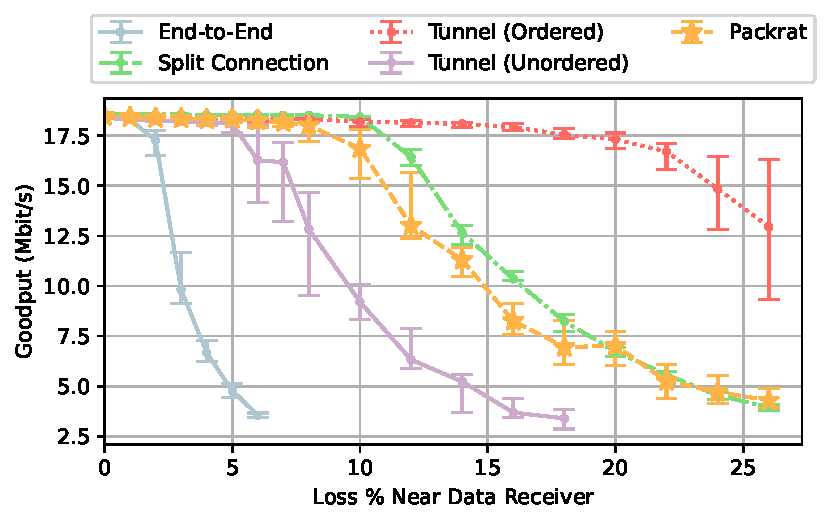
\includegraphics[width=\linewidth]{packrat/figures/http_benchmark.pdf}
        \caption{QUIC HTTP/3 file download.}
        \label{fig:packrat:perf:http}
    \end{subfigure}
    \begin{subfigure}[b]{0.48\linewidth}
        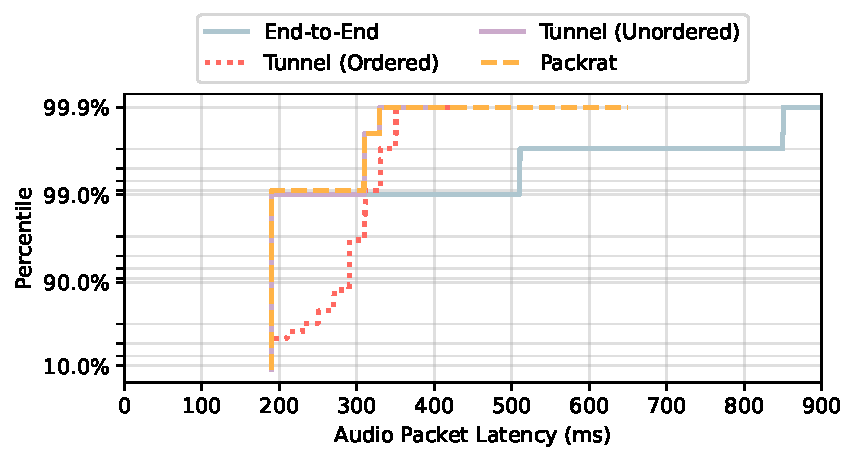
\includegraphics[width=\linewidth]{packrat/figures/media_benchmark.pdf}
        \caption{Low-latency media stream with FEC.}
        \label{fig:packrat:perf:media}
    \end{subfigure}
    \begin{subfigure}[b]{0.48\linewidth}
        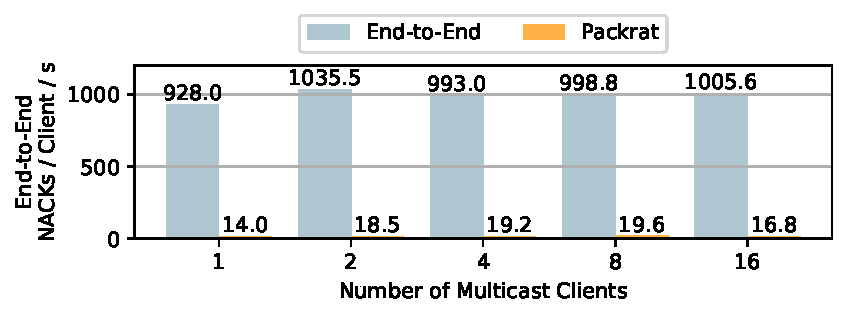
\includegraphics[width=\linewidth]{packrat/figures/multicast_benchmark.pdf}
        \caption{Reliable IP multicast stream.}
        \label{fig:packrat:perf:multicast}
    \end{subfigure}
    \caption{In-network retransmissions from the Packrat proxy enable applications
     to achieve better throughput, latency, and link
     overheads in lossy network settings compared to end-to-end
     retransmissions. Applications using the tunnel differ in whether they
     benefit based on the tunnel configuration, which is a disadvantage of
     link-layer retransmissions.}
    \label{fig:packrat:perf}
\end{figure}

We find that in-network retransmissions via the Packrat proxy enable a
variety of performance enhancements---higher throughput, lower latency, and
lower link overheads than end-to-end retransmissions---for a variety of
encrypted transport protocols when the data receiver is near a lossy path
segment (\Cref{fig:packrat:perf}). Our link-layer tunnels both harm and help
performance depending on their configurations, but they are transparent to the
applications that share the link.
% The Packrat protocol enables similar improvements to connection-splitting PEPs without ossifying the protocol. Unlike link-layer retransmissions, the Packrat protocol can be tailored to each application.
% The Packrat proxy is on-path and doesn't fate share with the application nor incur encapsulation overheads, unlike transport-layer tunnels.

\subsubsection{HTTP/3 file download.}
Packrat improves the throughput of a large HTTP/3 file download
$2.7\times$
% end-to-end 6.6720788246424245 at 4%
% packrat 18.30892838311422
% 18.3... / 6.67... = 2.744..
compared to end-to-end with 4\% loss on the near path segment
(\Cref{fig:packrat:perf:http}). End-to-end QUIC with CUBIC, in line with other
studies on ``loss-based'' congestion control, achieves poor link utilization in
even minimally lossy environments. While the performance of CCAs differ by
implementation, \texttt{picoquic} CUBIC has been shown to be one of the more
aggressive ones~\cite{yuan2025internet}.

QUIC with a Packrat achieves similar throughput to QUIC with an explicit
connection splitter as loss increases. They both utilize nearly all available
bandwidth until $\approx\!10\%$ loss, before gradually deteriorating. In the
split connection, this behavior is due to the congestion window on the near
path segment being able to compensate for high loss with a short delay, to a
certain threshold. With Packrat, this is because the reorder delay initially
hides loss from the congestion control algorithm at the data sender. As the
loss increases, we observe that the proxy fails to decode the quACK more often
and resets the connection. Each time there is a reset, the receiver falls back
to end-to-end retransmissions, signaling more loss (and congestion) to the data
sender. This suggests that the congestion response to loss with Packrat can be
both as good and as fair as QUIC with a connection splitter, without fate
sharing or decrypting the connection at the proxy.

For the HTTP/3 download in this low-latency, low-loss network setting, the
ordered tunnel outperforms QUIC with a Packrat. The unordered tunnel does not
perform as well because the retransmits at millisecond timesecales arrive
out-of-order. The end-to-end ACKs subsequently cause the server to send
spurious retransmissions (\Cref{fig:packrat:spurious:http}). The congestion response to
spurious retransmissions is not well-defined in standards, and \texttt
{picoquic} makes some attempt to revert the congestion window that leads to
this result, which is a similar result we observe when using Packrat with no
reorder signal. The ordered tunnel does not run into the same issues because
its aggressive retransmissions, when ordered, hide most loss the server could
interpret as a congestion signal.

\subsubsection{Low-latency media with FEC.}

Packrat enables fewer and shorter stalls in a low-latency media stream over a
high-delay satellite network (\Cref{fig:packrat:perf:media}). In this network setting,
the minimum one-way latency of a packet is already 190 ms (40 ms encoding + 150
ms delay). For reference, 150 ms is the normal latency for VoIP, and anything
above produces a noticeable drop in quality. Thus network-generated
retransmissions are crucial in lossy, high-latency settings.

Both Packrat and end-to-end benefit from FEC, but Packrat enables shorter stalls when
a frame still needs to be retransmitted. In this transport protocol, a frame
needs to be retransmitted if two packets are lost in a row. Thus at 10\% loss,
the 99th percentile delay of both mechanisms is the minimum of 190 ms. In the
remaining percentile, one more out-of-order packet arrives after $20$ ms,
draining the last of the buffer and generating a quACK or NACK. The length of
the stall is then the 100 or 300 ms RTT with the proxy or server. The unordered
tunnel exhibits a similar behavior to Packrat.

Unlike the HTTP/3 benchmark, this transport protocol gets none of the benefits
of FEC with the \textit{ordered} tunnel. When a retransmission is required, the
tunnel buffers at least 6 more packets until it receives the retransmission and
releases them to the client. The buffering causes unnecessary stalls. If the
tunnel had just released the packets, a single missing packet would have been
masked by the repetition code.

\subsubsection{Reliable IP multicast stream.}

Caching packets in the network like a CDN is inherently beneficial because it
can reduce the congestion in the core network. This is one of the idealistic
draws of IP multicast, but it is rarely used over the Internet in practice
because a reliable stream may require an overwhelming number of unicast
retransmissions from the server when there is loss. While CDNs and SFUs have
helped with content distribution, these are not options for encrypted transport
protocols without embedding trust in the network.

The Packrat proxy can handle in-network retransmissions for a large number of
multicast clients. Each client using the Packrat proxy sends on average $16.8$
end-to-end retransmissions/second, a $59\!\times$ reduction from $1005.6$
retransmissions/second/client without Packrat (\Cref{fig:packrat:perf:multicast}).
This reduction scales with the
number of clients. In-network retransmissions reduce both the load at the
server and congestion in the network.\\

\noindent
The behaviors of the QUIC and media transport protocols with various tunnels
represent the challenges of configuring link-layer retransmissions
independently of the applications that share the link. A large download
over QUIC performs poorly
when there is excessive reordering, while the media transport protocol prefers
to receive packets right away.
Disabling link-layer retransmissions introduces loss, which can be even more
detrimental for performance.

\subsection{Link overheads using rateless and sparse quACKing}
\label{sec:packrat:emulation:link-overheads}

\begin{figure*}[ht]
\centering
\begin{minipage}[t]{0.3\textwidth}
    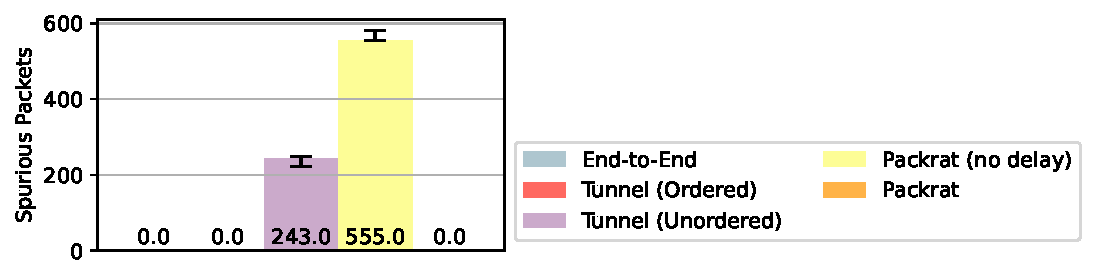
\includegraphics[width=\linewidth, trim=245 15 5 65, clip]{packrat/figures/spurious_retx_legend.pdf}
    \begin{subfigure}[b]{\linewidth}
        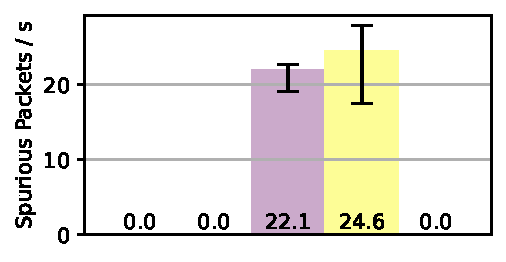
\includegraphics[width=\linewidth]{packrat/figures/spurious_retx_http.pdf}
        \caption{HTTP/3 download.}
        \label{fig:packrat:spurious:http}
    \end{subfigure}
    \begin{subfigure}[b]{\linewidth}
        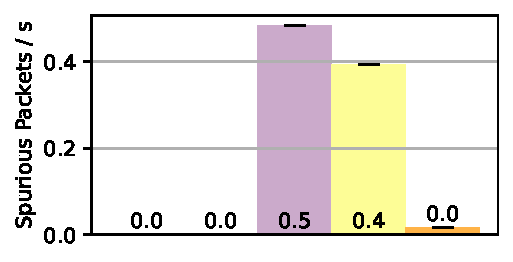
\includegraphics[width=\linewidth]{packrat/figures/spurious_retx_media.pdf}
        \caption{Low-latency media.}
        \label{fig:packrat:spurious:media}
    \end{subfigure}
    \caption{The unordered tunnel and Packrat without modifying the end-to-end
     reorder delay cause the client to receive spurious retransmissions.
     Adding a reorder delay with Packrat significantly reduces them.}
    \label{fig:packrat:spurious}
\end{minipage}%
\hfill
\begin{minipage}[t]{0.68\textwidth}
    \centering
    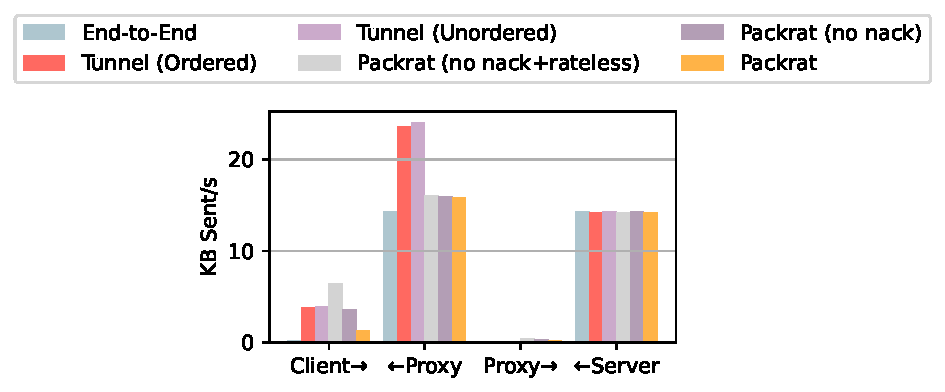
\includegraphics[width=0.9\linewidth, trim=5 140 5 5, clip]{packrat/figures/network_stats_media_legend.pdf}
    
    \begin{subfigure}[b]{0.48\linewidth}
        \centering
        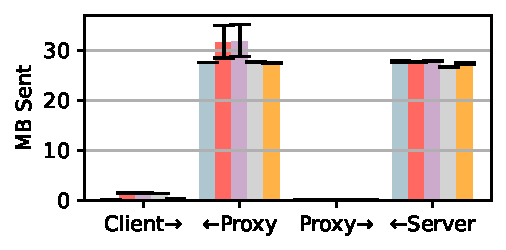
\includegraphics[width=\linewidth]{packrat/figures/network_stats_http_tx_bytes.pdf}
        \caption{HTTP/3 download (bytes).}
        \label{fig:packrat:link-overheads:http-bytes}
    \end{subfigure}
    \begin{subfigure}[b]{0.51\linewidth}
        \centering
        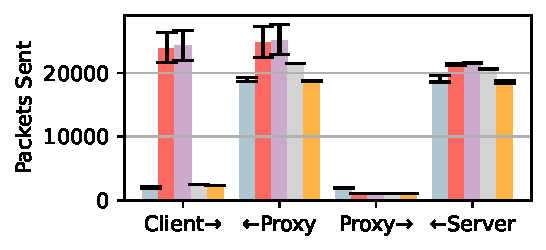
\includegraphics[width=\linewidth]{packrat/figures/network_stats_http_tx_packets.pdf}
        \caption{HTTP/3 download (packets).}
        \label{fig:packrat:link-overheads:http-packets}
    \end{subfigure}\\

    \begin{subfigure}[b]{0.49\linewidth}
        \centering
        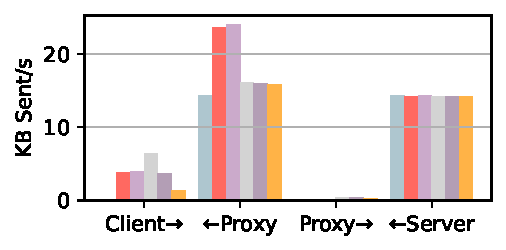
\includegraphics[width=\linewidth]{packrat/figures/network_stats_media_tx_bytes.pdf}
        \caption{Low-latency media (bytes).}
        \label{fig:packrat:link-overheads:media-bytes}
    \end{subfigure}
    \begin{subfigure}[b]{0.49\linewidth}
        \centering
        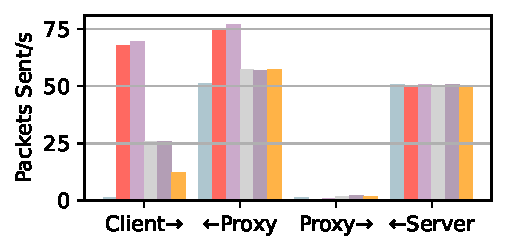
\includegraphics[width=\linewidth]{packrat/figures/network_stats_media_tx_packets.pdf}
        \caption{Low-latency media (packets).}
        \label{fig:packrat:link-overheads:media-packets}
    \end{subfigure}
    
    \caption{The number of bytes (left) and packets (right) sent between the
     client, proxy, and server. The statistics are captured directly from the
     network interface. The link overheads from quACKs using the Packrat proxy are
     comparable to those of the underlying acknowledgment scheme. The client
     sends fewer bytes with rateless quACKs, and fewer packets with sparse
     quACKing. The tunnel aggressively ACKs and retransmits.}
    \label{fig:packrat:link-overheads}
\end{minipage}
\end{figure*}

In this section, we analyze how sending quACKs with the optimizations in \Cref
{sec:packrat:receiver:rateless} impacts the link overheads in the network.
\Cref{fig:packrat:link-overheads} displays the number of packets and bytes sent on each
link between the client, proxy, and server in the HTTP and media applications.
As a proportion of the volume in bytes sent by both endpoints of the
application, the HTTP client makes up $1.3\%$ of the traffic with Packrat and
$0.7\%$ without. The media client makes up $8.2\%$ of the traffic with Packrat
and $1.0\%$ without. We find that that we can reasonably think of quACKs as
control packets in the common case.

\subsubsection{Rateless quACKs.}
Using the rateless property to send smaller quACKs
reduces the number of bytes the client sends by $3.6\!\times$ (\Cref
{fig:packrat:link-overheads:http-bytes}) and $1.8\!\times$ (\Cref
{fig:packrat:link-overheads:media-bytes}) compared to Packrat without the optimization.
% http sender tx_bytes 1266149.5 -> 351208.0
% 1266149.5/351208.0=3.6x
% media sender tx_bytes 6397.578993802214 -> 3632.7542920194414 -> 1.8x
This property allows clients to configure the number of symbols less
conservatively when initializing the Packrat connection while being able to
dynamically adjust to changing loss conditions, particularly in less controlled
non-emulation environments.

\subsubsection{Sending quACKs on NACK.}

% media sender tx_packets 25.786554138093248 -> 12.33599987063784
Sending a quACK only when the client would otherwise send a NACK reduces the
number of packets the media client sends $1.9\!\times$ (\Cref
{fig:packrat:link-overheads:media-packets}). Note that without sending on NACK, we
configured the media client to quACK every other packet to balance latency with
frequent quACKing. The media client sends more packets than end-to-end because
although it only ACKs when there is a missing \textit{frame}, it quACKs when
there is a missing \textit{packet} because the FEC is opaque to the proxy.
% media sender tx_bytes 1275.1961129433735 -> 147.66572118181435
% 1127.53 * 8 = 9 Kbit

\subsubsection{Base connection improvements.}

Even though the HTTP client quACKs at a similar frequency to which it ACKs, the
client sends a similar number of packets with and without the Packrat (\Cref
{fig:packrat:link-overheads:http-packets}). The proxy in the end-to-end scenario sends
nearly twice as many ACKs to the server because the number of ACKs depends on
the length of the connection. Packrat improves the throughput so much that the
number of net packets sent by the client are similar.

The IP multicast application demonstrates how Packrat can reduce congestion closer
to the server by caching retransmissions in the middle of the network (\Cref
{fig:packrat:perf:multicast}). This is especially impactful if the data is shared by
multiple clients.\\

\noindent Note that the tunnels aggressively ACK and retransmit in both
directions. The client sends $12$-$66\!\times$ additional packets compared to
end-to-end and the proxy sends $33$-$51$\% more to the client. Even though the
block ACKs are small, it can be costly for radios to switch often between
sending and receiving modes, and for proxies with per-packet overheads.

\subsection{CPU overheads of decoding at the proxy}
\label{sec:packrat:emulation:cpu-overheads}

In this experiment, we analyze the number of cycles that the proxy
needs to process each
packet in the HTTP/3 benchmark, and use the per-packet overheads to extrapolate
the maximum processing capacity of a CPU-constrained proxy. These overheads
include both quACK operations and transport-protocol logic for, e.g.,
packet triaging, loss detection, and cache management.

Each data packet on the base connection takes on average $1002$ cycles/packet.
The main overhead comes from adding the packet to a ring buffer used as the
packet cache.

Each quACK on the Packrat connection takes on average 27716 cycles/packet. The
proxy determines which packets to retransmit based on the quACK and evicts
packets. Loss detection involves encoding a delta of packets since the last
quACK into the existing state, as well as decoding the received quACK. Encoding
uses a total of $7156/27716 = 25.8\%$ of the cycles and decoding $3560/27716 =
12.8\%$. With a total of $38.6\%$ of the processing time spent on IBLT
operations, this implies that both encoding and decoding are valuable to optimize.

% psum
% WARN [proxy::cycles] transport
% WARN [proxy::cycles] 953 (total=101000,prop=1.000)
% WARN [proxy::cycles] transport,encode,decode
% WARN [proxy::cycles] 32923,9572,2984 (total=6800,prop=1.000,1.000,0.789)

% iblt
% WARN [proxy::cycles] transport
% WARN [proxy::cycles] 1002 (total=101000,prop=1.000)
% WARN [proxy::cycles] transport,encode,decode
% WARN [proxy::cycles] 27716,7156,3560 (total=6200,prop=1.000,1.000,0.516)

In this application, there is approximately one quACK for every $16.3$ data
packets. If each data packet uses a full MTU of 1500 bytes, this means a single
core of a 2.4 GHz CPU on a proxy would theoretically be able to handle 10.7
Gbit/s\footnote{ $2.4\text{ Gcycles/s }
\times(16.3 \text{ data packets } / (27716\cdot1 + 1002\cdot16.3) \text{ cycles })
\times (1500 \text{ bytes/data packet })
\times (8 \text{ bits/byte })
= 10.7 \text{ Gbit/s}$.
}. However, this estimate does not account for the substantial CPU overhead
involved in reading and writing to the NIC---these can be significantly reduced
using kernel bypass frameworks like DPDK or with specialized networking
hardware.

% iblt
% 2.4 Gcycles/s
% * 16.29 data packets / (27716*1 + 1002*16.29) cycles
% * 1500 bytes / data packet
% * 8 bits / 1 byte
% = 10.7 Gbit/s.

% psum
% 2.4 Gcycles/s
% * 14.85 data packets / (32923*1 + 953*14.85) cycles
% * 1500 bytes / data packet
% * 8 bits / 1 byte
% = 11.2 Gbit/s

\subsection{Memory overheads of the proxy cache}
\label{sec:packrat:emulation:memory-overheads}

\begin{figure}[t]
    \centering
    \begin{subfigure}[b]{0.49\linewidth}
        \centering
        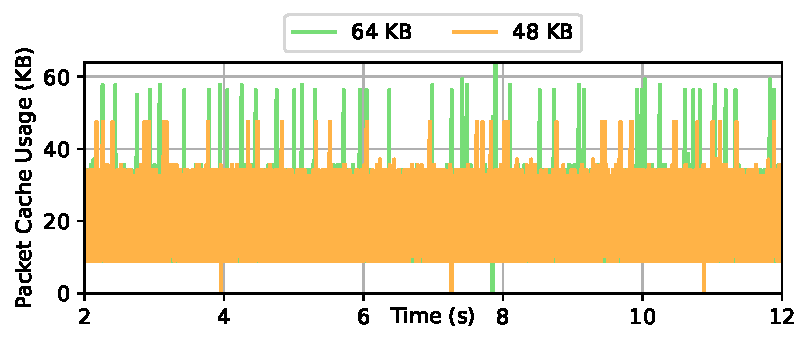
\includegraphics[width=\linewidth]{packrat/figures/cache_http.pdf}
        \caption{HTTP/3 file download.
        % \thea{May be a non-issue, but not sure how to interpret the mass of orange here.}
        }
        \label{fig:packrat:memory:http}
    \end{subfigure}
    \begin{subfigure}[b]{0.49\linewidth}
        \centering
        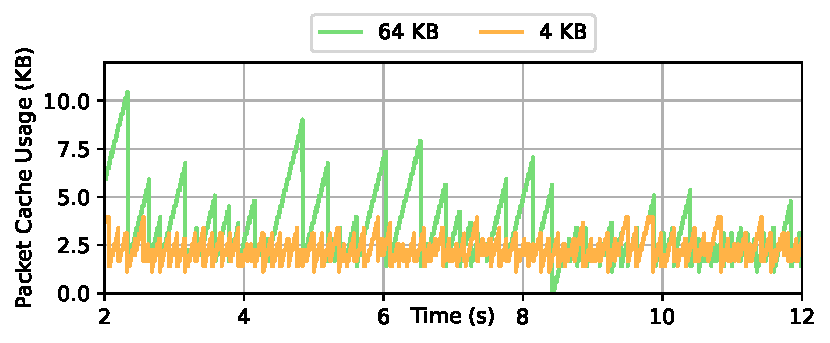
\includegraphics[width=\linewidth]{packrat/figures/cache_media.pdf}
        \caption{Low-latency media with FEC.}
        \label{fig:packrat:memory:media}
    \end{subfigure}
    \caption{The number of bytes in the cache over a
     10-second period with both bounded (48 KB or 4 KB) and unbounded (64 KB)
     cache sizes. The proxy uses optimistic eviction if an incoming packet
     causes the cache to exceed its capacity.}
    \label{fig:packrat:memory}
\end{figure}

\begin{figure}[t]
    \centering
    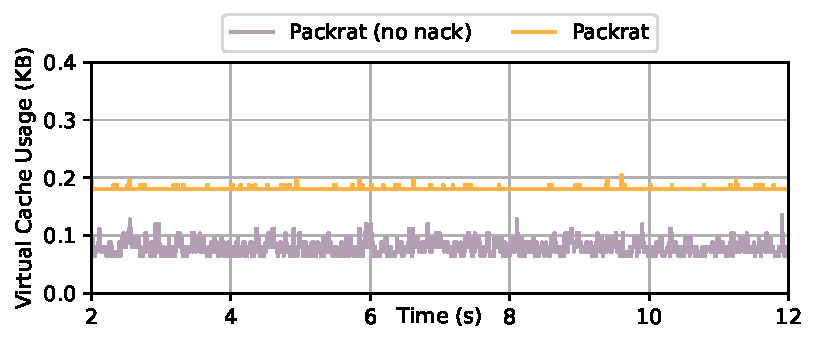
\includegraphics[width=0.6\linewidth]{packrat/figures/cache_multicast.pdf}
    \caption{The sum of the virtual cache sizes of all $16$ clients in
     the multicast application. Each client uses $\approx\!$12 bytes each for a
     single insertion pair. The variations are due to individuals having
     slightly more or less than one insertion pair. Without sparse quACKing
     (``no nack''), clients more often have empty virtual buffers. The base
     connection's packet cache (not pictured) is always 64 KB.}
    \label{fig:packrat:memory:multicast}
\end{figure}

We find that the Packrat proxy needs no more memory
than similar proxies for unencrypted transport protocols, and that the optimistic
eviction policy is an effective fallback for when the cache exceeds its memory limits.
Like any in-network retransmission mechanism,
the most significant memory usage at the proxy comes from the packet
cache. \Cref{fig:packrat:memory} shows the number of bytes in the packet contents of
the cache over a 10-second period of each application in our chosen
network settings. The maximum cache size
at the Packrat proxy is 64kB per connection, similar to a typical TCP window size.

\subsubsection{HTTP/3 file download.}

The cache grows quickly because each data packet is large, but evicts
packets every 10~ms when
it receives a quACK (\Cref{fig:packrat:memory:http}). The minimum cache size is
$\approx\!10$ kB, the size of the outstanding packets between the client and
proxy. A spike occurs when a quACK is dropped, at which point the proxy
optimistically evicts. The proxy resets the connection if there is an
error, which is more common with a smaller cache, and drops the cache
size to 0.

\subsubsection{Low-latency media with FEC.}

The media application relies on optimistic eviction to keep the cache small
since the client sparsely quACKs (\Cref{fig:packrat:memory:media}). The
line plateaus at the maximum cache size because the proxy
assumes these packets have been received. The cache size only needs to fit 1-2
RTTs of packets between the client and proxy.

\subsubsection{Reliable IP multicast stream.}

The multicast application has a fixed packet cache size of 64 kB, and we analyze
the memory overheads of the per-client virtual caches (\Cref{fig:packrat:memory:multicast}).
In particular, we calculate the overhead of each virtual cache as 4 bytes for
the first global index and then 8 bytes for each insertion pair
(\Cref{sec:packrat:implementation:proxy}). When there are 16 clients, the proxy
uses on average 0.178 KB in the virtual caches for a very low overhead of 12
bytes/client. That is exactly one insertion pair, and in general the overheads
of the virtual caches are proportional to the number of outstanding
retransmissions.
% average = 0.17788111888111888 KB = 1

\section{Summary}
\label{sec:packrat:summary}

In this chapter, we described and evaluated the Packrat proxy for sending
network-originated retransmissions when the end-to-end transport is encrypted.
We use set-reconciliation techniques based on the Rateless IBLT to let the
receiver efficiently acknowledge encrypted packets, yielding performance
benefits in lossy settings without an additional layer of encapsulation,
tunnel, or link-layer retransmissions.
